
%% bare_conf.tex
%% V1.4a
%% 2014/09/17
%% by Michael Shell
%% See:
%% http://www.michaelshell.org/
%% for current contact information.
%%
%% This is a skeleton file demonstrating the use of IEEEtran.cls
%% (requires IEEEtran.cls version 1.8a or later) with an IEEE
%% conference paper.
%%
%% Support sites:
%% http://www.michaelshell.org/tex/ieeetran/
%% http://www.ctan.org/tex-archive/macros/latex/contrib/IEEEtran/
%% and
%% http://www.ieee.org/

%%*************************************************************************
%% Legal Notice:
%% This code is offered as-is without any warranty either expressed or
%% implied; without even the implied warranty of MERCHANTABILITY or
%% FITNESS FOR A PARTICULAR PURPOSE! 
%% User assumes all risk.
%% In no event shall IEEE or any contributor to this code be liable for
%% any damages or losses, including, but not limited to, incidental,
%% consequential, or any other damages, resulting from the use or misuse
%% of any information contained here.
%%
%% All comments are the opinions of their respective authors and are not
%% necessarily endorsed by the IEEE.
%%
%% This work is distributed under the LaTeX Project Public License (LPPL)
%% ( http://www.latex-project.org/ ) version 1.3, and may be freely used,
%% distributed and modified. A copy of the LPPL, version 1.3, is included
%% in the base LaTeX documentation of all distributions of LaTeX released
%% 2003/12/01 or later.
%% Retain all contribution notices and credits.
%% ** Modified files should be clearly indicated as such, including  **
%% ** renaming them and changing author support contact information. **
%%
%% File list of work: IEEEtran.cls, IEEEtran_HOWTO.pdf, bare_adv.tex,
%%                    bare_conf.tex, bare_jrnl.tex, bare_conf_compsoc.tex,
%%                    bare_jrnl_compsoc.tex, bare_jrnl_transmag.tex
%%*************************************************************************


% *** Authors should verify (and, if needed, correct) their LaTeX system  ***
% *** with the testflow diagnostic prior to trusting their LaTeX platform ***
% *** with production work. IEEE's font choices and paper sizes can       ***
% *** trigger bugs that do not appear when using other class files.       ***                          ***
% The testflow support page is at:
% http://www.michaelshell.org/tex/testflow/



\documentclass[conference]{Trabalho_1}
\usepackage{graphicx, url, epsfig, subfigure}
\usepackage{amsmath, amscd, amsthm, amsxtra}

\usepackage[brazil]{babel}   
\usepackage[latin1]{inputenc}
\usepackage{listings}
\usepackage{color}
% Some Computer Society conferences also require the compsoc mode option,
% but others use the standard conference format.
%
% If IEEEtran.cls has not been installed into the LaTeX system files,
% manually specify the path to it like:
% \documentclass[conference]{../sty/IEEEtran}





% Some very useful LaTeX packages include:2
% (uncomment the ones you want to load)


% *** MISC UTILITY PACKAGES ***
%
%\usepackage{ifpdf}
% Heiko Oberdiek's ifpdf.sty is very useful if you need conditional
% compilation based on whether the output is pdf or dvi.
% usage:
% \ifpdf
%   % pdf code
% \else
%   % dvi code
% \fi
% The latest version of ifpdf.sty can be obtained from:
% http://www.ctan.org/tex-archive/macros/latex/contrib/oberdiek/
% Also, note that IEEEtran.cls V1.7 and later provides a builtin
% \ifCLASSINFOpdf conditional that works the same way.
% When switching from latex to pdflatex and vice-versa, the compiler may
% have to be run twice to clear warning/error messages.






% *** CITATION PACKAGES ***
%
%\usepackage{cite}
% cite.sty was written by Donald Arseneau
% V1.6 and later of IEEEtran pre-defines the format of the cite.sty package
% \cite{} output to follow that of IEEE. Loading the cite package will
% result in citation numbers being automatically sorted and properly
% "compressed/ranged". e.g., [1], [9], [2], [7], [5], [6] without using
% cite.sty will become [1], [2], [5]--[7], [9] using cite.sty. cite.sty's
% \cite will automatically add leading space, if needed. Use cite.sty's
% noadjust option (cite.sty V3.8 and later) if you want to turn this off
% such as if a citation ever needs to be enclosed in parenthesis.
% cite.sty is already installed on most LaTeX systems. Be sure and use
% version 5.0 (2009-03-20) and later if using hyperref.sty.
% The latest version can be obtained at:
% http://www.ctan.org/tex-archive/macros/latex/contrib/cite/
% The documentation is contained in the cite.sty file itself.






% *** GRAPHICS RELATED PACKAGES ***
%
\ifCLASSINFOpdf
  % \usepackage[pdftex]{graphicx}
  % declare the path(s) where your graphic files are
  % \graphicspath{{../pdf/}{../jpeg/}}
  % and their extensions so you won't have to specify these with
  % every instance of \includegraphics
  % \DeclareGraphicsExtensions{.pdf,.jpeg,.png}
\else
  % or other class option (dvipsone, dvipdf, if not using dvips). graphicx
  % will default to the driver specified in the system graphics.cfg if no
  % driver is specified.
  % \usepackage[dvips]{graphicx}
  % declare the path(s) where your graphic files are
  % \graphicspath{{../eps/}}
  % and their extensions so you won't have to specify these with
  % every instance of \includegraphics
  % \DeclareGraphicsExtensions{.eps}
\fi
% graphicx was written by David Carlisle and Sebastian Rahtz. It is
% required if you want graphics, photos, etc. graphicx.sty is already
% installed on most LaTeX systems. The latest version and documentation
% can be obtained at: 
% http://www.ctan.org/tex-archive/macros/latex/required/graphics/
% Another good source of documentation is "Using Imported Graphics in
% LaTeX2e" by Keith Reckdahl which can be found at:
% http://www.ctan.org/tex-archive/info/epslatex/
%
% latex, and pdflatex in dvi mode, support graphics in encapsulated
% postscript (.eps) format. pdflatex in pdf mode supports graphics
% in .pdf, .jpeg, .png and .mps (metapost) formats. Users should ensure
% that all non-photo figures use a vector format (.eps, .pdf, .mps) and
% not a bitmapped formats (.jpeg, .png). IEEE frowns on bitmapped formats
% which can result in "jaggedy"/blurry rendering of lines and letters as
% well as large increases in file sizes.
%
% You can find documentation about the pdfTeX application at:
% http://www.tug.org/applications/pdftex





% *** MATH PACKAGES ***
%
%\usepackage[cmex10]{amsmath}
% A popular package from the American Mathematical Society that provides
% many useful and powerful commands for dealing with mathematics. If using
% it, be sure to load this package with the cmex10 option to ensure that
% only type 1 fonts will utilized at all point sizes. Without this option,
% it is possible that some math symbols, particularly those within
% footnotes, will be rendered in bitmap form which will result in a
% document that can not be IEEE Xplore compliant!
%
% Also, note that the amsmath package sets \interdisplaylinepenalty to 10000
% thus preventing page breaks from occurring within multiline equations. Use:
%\interdisplaylinepenalty=2500
% after loading amsmath to restore such page breaks as IEEEtran.cls normally
% does. amsmath.sty is already installed on most LaTeX systems. The latest
% version and documentation can be obtained at:
% http://www.ctan.org/tex-archive/macros/latex/required/amslatex/math/





% *** SPECIALIZED LIST PACKAGES ***
%
%\usepackage{algorithmic}
% algorithmic.sty was written by Peter Williams and Rogerio Brito.
% This package provides an algorithmic environment fo describing algorithms.
% You can use the algorithmic environment in-text or within a figure
% environment to provide for a floating algorithm. Do NOT use the algorithm
% floating environment provided by algorithm.sty (by the same authors) or
% algorithm2e.sty (by Christophe Fiorio) as IEEE does not use dedicated
% algorithm float types and packages that provide these will not provide
% correct IEEE style captions. The latest version and documentation of
% algorithmic.sty can be obtained at:
% http://www.ctan.org/tex-archive/macros/latex/contrib/algorithms/
% There is also a support site at:
% http://algorithms.berlios.de/index.html
% Also of interest may be the (relatively newer and more customizable)
% algorithmicx.sty package by Szasz Janos:
% http://www.ctan.org/tex-archive/macros/latex/contrib/algorithmicx/




% *** ALIGNMENT PACKAGES ***
%
%\usepackage{array}
% Frank Mittelbach's and David Carlisle's array.sty patches and improves
% the standard LaTeX2e array and tabular environments to provide better
% appearance and additional user controls. As the default LaTeX2e table
% generation code is lacking to the point of almost being broken with
% respect to the quality of the end results, all users are strongly
% advised to use an enhanced (at the very least that provided by array.sty)
% set of table tools. array.sty is already installed on most systems. The
% latest version and documentation can be obtained at:
% http://www.ctan.org/tex-archive/macros/latex/required/tools/


% IEEEtran contains the IEEEeqnarray family of commands that can be used to
% generate multiline equations as well as matrices, tables, etc., of high
% quality.




% *** SUBFIGURE PACKAGES ***
%\ifCLASSOPTIONcompsoc
%  \usepackage[caption=false,font=normalsize,labelfont=sf,textfont=sf]{subfig}
%\else
%  \usepackage[caption=false,font=footnotesize]{subfig}
%\fi
% subfig.sty, written by Steven Douglas Cochran, is the modern replacement
% for subfigure.sty, the latter of which is no longer maintained and is
% incompatible with some LaTeX packages including fixltx2e. However,
% subfig.sty requires and automatically loads Axel Sommerfeldt's caption.sty
% which will override IEEEtran.cls' handling of captions and this will result
% in non-IEEE style figure/table captions. To prevent this problem, be sure
% and invoke subfig.sty's "caption=false" package option (available since
% subfig.sty version 1.3, 2005/06/28) as this is will preserve IEEEtran.cls
% handling of captions.
% Note that the Computer Society format requires a larger sans serif font
% than the serif footnote size font used in traditional IEEE formatting
% and thus the need to invoke different subfig.sty package options depending
% on whether compsoc mode has been enabled.
%
% The latest version and documentation of subfig.sty can be obtained at:
% http://www.ctan.org/tex-archive/macros/latex/contrib/subfig/




% *** FLOAT PACKAGES ***
%
%\usepackage{fixltx2e}
% fixltx2e, the successor to the earlier fix2col.sty, was written by
% Frank Mittelbach and David Carlisle. This package corrects a few problems
% in the LaTeX2e kernel, the most notable of which is that in current
% LaTeX2e releases, the ordering of single and double column floats is not
% guaranteed to be preserved. Thus, an unpatched LaTeX2e can allow a
% single column figure to be placed prior to an earlier double column
% figure. The latest version and documentation can be found at:
% http://www.ctan.org/tex-archive/macros/latex/base/


%\usepackage{stfloats}
% stfloats.sty was written by Sigitas Tolusis. This package gives LaTeX2e
% the ability to do double column floats at the bottom of the page as well
% as the top. (e.g., "\begin{figure*}[!b]" is not normally possible in
% LaTeX2e). It also provides a command:
%\fnbelowfloat
% to enable the placement of footnotes below bottom floats (the standard
% LaTeX2e kernel puts them above bottom floats). This is an invasive package
% which rewrites many portions of the LaTeX2e float routines. It may not work
% with other packages that modify the LaTeX2e float routines. The latest
% version and documentation can be obtained at:
% http://www.ctan.org/tex-archive/macros/latex/contrib/sttools/
% Do not use the stfloats baselinefloat ability as IEEE does not allow
% \baselineskip to stretch. Authors submitting work to the IEEE should note
% that IEEE rarely uses double column equations and that authors should try
% to avoid such use. Do not be tempted to use the cuted.sty or midfloat.sty
% packages (also by Sigitas Tolusis) as IEEE does not format its papers in
% such ways.
% Do not attempt to use stfloats with fixltx2e as they are incompatible.
% Instead, use Morten Hogholm'a dblfloatfix which combines the features
% of both fixltx2e and stfloats:
%
% \usepackage{dblfloatfix}
% The latest version can be found at:
% http://www.ctan.org/tex-archive/macros/latex/contrib/dblfloatfix/




% *** PDF, URL AND HYPERLINK PACKAGES ***
%
%\usepackage{url}
% url.sty was written by Donald Arseneau. It provides better support for
% handling and breaking URLs. url.sty is already installed on most LaTeX
% systems. The latest version and documentation can be obtained at:
% http://www.ctan.org/tex-archive/macros/latex/contrib/url/
% Basically, \url{my_url_here}.




% *** Do not adjust lengths that control margins, column widths, etc. ***
% *** Do not use packages that alter fonts (such as pslatex).         ***
% There should be no need to do such things with IEEEtran.cls V1.6 and later.
% (Unless specifically asked to do so by the journal or conference you plan
% to submit to, of course. )


% correct bad hyphenation here
\hyphenation{op-tical net-works semi-conduc-tor}


\begin{document}
%
% paper title
% Titles are generally capitalized except for words such as a, an, and, as,
% at, but, by, for, in, nor, of, on, or, the, to and up, which are usually
% not capitalized unless they are the first or last word of the title.
% Linebreaks \\ can be used within to get better formatting as desired.
% Do not put math or special symbols in the title.
\title{Detec\c{c}\~ao de Componentes Conectados e Classifica\c{c}\~ao de Imagens}


% author names and affiliations
% use a multiple column layout for up to three different
% affiliations
\author{\IEEEauthorblockN{Rodrigo Ferreira Guimar\~aes}
\IEEEauthorblockA{Departamento de Ci\^encia de Computa\c{c}\~ao e Faculdade de Tecnologia\\
Universidade de Bras\'ilia, Bras\'ilia\\
Email: rodrigofegui@aluno.unb.br}
}

% conference papers do not typically use \thanks and this command
% is locked out in conference mode. If really needed, such as for
% the acknowledgment of grants, issue a \IEEEoverridecommandlockouts
% after \documentclass

% for over three affiliations, or if they all won't fit within the width
% of the page, use this alternative format:
% 
%\author{\IEEEauthorblockN{Michael Shell\IEEEauthorrefmark{1},
%Homer Simpson\IEEEauthorrefmark{2},
%James Kirk\IEEEauthorrefmark{3}, 
%Montgomery Scott\IEEEauthorrefmark{3} and
%Eldon Tyrell\IEEEauthorrefmark{4}}
%\IEEEauthorblockA{\IEEEauthorrefmark{1}School of Electrical and Computer Engineering\\
%Georgia Institute of Technology,
%Atlanta, Georgia 30332--0250\\ Email: see http://www.michaelshell.org/contact.html}
%\IEEEauthorblockA{\IEEEauthorrefmark{2}Twentieth Century Fox, Springfield, USA\\
%Email: homer@thesimpsons.com}
%\IEEEauthorblockA{\IEEEauthorrefmark{3}Starfleet Academy, San Francisco, California 96678-2391\\
%Telephone: (800) 555--1212, Fax: (888) 555--1212}
%\IEEEauthorblockA{\IEEEauthorrefmark{4}Tyrell Inc., 123 Replicant Street, Los Angeles, California 90210--4321}}




% use for special paper notices
%\IEEEspecialpapernotice{(Invited Paper)}




% make the title area
\maketitle

% As a general rule, do not put math, special symbols or citations
% in the abstract
\begin{abstract}
The abstract goes here.
\end{abstract}

% no keywords




% For peer review papers, you can put extra information on the cover
% page as needed:
% \ifCLASSOPTIONpeerreview
% \begin{center} \bfseries EDICS Category: 3-BBND \end{center}
% \fi
%
% For peerreview papers, this IEEEtran command inserts a page break and
% creates the second title. It will be ignored for other modes.
\IEEEpeerreviewmaketitle



\section{Introdu\c{c}\~ao}
Este trabalho trata da detec\c{c}\~ao de componentes conectados e da classifica\c{c}\~ao de imagens, a partir desta detec\c{c}\~ao. Foi constru\'ido, com o aux\'ilio da toda a turma, um banco de dados com mais de $200$ imagens, sendo estas divididas igualmente em duas classes:~\textbf{classe 1} compreende as imagens que possuem pessoas com a maior parte do corpo exposta; enquanto que para a~\textbf{classe 2} compreende as imagens com as pessoas vestidas.

O trabalho objetiva realizar:~\textbf{a)} a binariza\c{c}\~ao das imagens a partir da segmenta\c{c}\~ao por cor de pele;~\textbf{b)} a rotula\c{c}\~ao para detectar a quantidade de elementos conectados na imagem bin\'aria;~\textbf{c)} a diferencia\c{c}\~ao do maior elemento conectado, atrav\'es da sua \'area; e por fim, ~\textbf{d)} a classifica\c{c}\~ao das imagens dentre as op\c{c}\~oes de classes.

 
\hfill 12 de Setembro, 2015


% An example of a floating figure using the graphicx package.
% Note that \label must occur AFTER (or within) \caption.
% For figures, \caption should occur after the \includegraphics.
% Note that IEEEtran v1.7 and later has special internal code that
% is designed to preserve the operation of \label within \caption
% even when the captionsoff option is in effect. However, because
% of issues like this, it may be the safest practice to put all your
% \label just after \caption rather than within \caption{}.
%
% Reminder: the "draftcls" or "draftclsnofoot", not "draft", class
% option should be used if it is desired that the figures are to be
% displayed while in draft mode.
%
%\begin{figure}[!t]
%\centering
%\includegraphics[width=2.5in]{myfigure}
% where an .eps filename suffix will be assumed under latex, 
% and a .pdf suffix will be assumed for pdflatex; or what has been declared
% via \DeclareGraphicsExtensions.
%\caption{Simulation results for the network.}
%\label{fig_sim}
%\end{figure}

% Note that IEEE typically puts floats only at the top, even when this
% results in a large percentage of a column being occupied by floats.


% An example of a double column floating figure using two subfigures.
% (The subfig.sty package must be loaded for this to work.)
% The subfigure \label commands are set within each subfloat command,
% and the \label for the overall figure must come after \caption.
% \hfil is used as a separator to get equal spacing.
% Watch out that the combined width of all the subfigures on a 
% line do not exceed the text width or a line break will occur.
%
%\begin{figure*}[!t]
%\centering
%\subfloat[Case I]{\includegraphics[width=2.5in]{box}%
%\label{fig_first_case}}
%\hfil
%\subfloat[Case II]{\includegraphics[width=2.5in]{box}%
%\label{fig_second_case}}
%\caption{Simulation results for the network.}
%\label{fig_sim}
%\end{figure*}
%
% Note that often IEEE papers with subfigures do not employ subfigure
% captions (using the optional argument to \subfloat[]), but instead will
% reference/describe all of them (a), (b), etc., within the main caption.
% Be aware that for subfig.sty to generate the (a), (b), etc., subfigure
% labels, the optional argument to \subfloat must be present. If a
% subcaption is not desired, just leave its contents blank,
% e.g., \subfloat[].


% An example of a floating table. Note that, for IEEE style tables, the
% \caption command should come BEFORE the table and, given that table
% captions serve much like titles, are usually capitalized except for words
% such as a, an, and, as, at, but, by, for, in, nor, of, on, or, the, to
% and up, which are usually not capitalized unless they are the first or
% last word of the caption. Table text will default to \footnotesize as
% IEEE normally uses this smaller font for tables.
% The \label must come after \caption as always.
%
%\begin{table}[!t]
%% increase table row spacing, adjust to taste
%\renewcommand{\arraystretch}{1.3}
% if using array.sty, it might be a good idea to tweak the value of
% \extrarowheight as needed to properly center the text within the cells
%\caption{An Example of a Table}
%\label{table_example}
%\centering
%% Some packages, such as MDW tools, offer better commands for making tables
%% than the plain LaTeX2e tabular which is used here.
%\begin{tabular}{|c||c|}
%\hline
%One & Two\\
%\hline
%Three & Four\\
%\hline
%\end{tabular}
%\end{table}


% Note that the IEEE does not put floats in the very first column
% - or typically anywhere on the first page for that matter. Also,
% in-text middle ("here") positioning is typically not used, but it
% is allowed and encouraged for Computer Society conferences (but
% not Computer Society journals). Most IEEE journals/conferences use
% top floats exclusively. 
% Note that, LaTeX2e, unlike IEEE journals/conferences, places
% footnotes above bottom floats. This can be corrected via the
% \fnbelowfloat command of the stfloats package.


\section{Embasamento Te\'orico}
Para que haja um correto entendimento sobre o desenvolvimento deste projeto \'e importante abordar alguns aspectos relevantes, como as defini\c{c}\~oes: de uma imagem; das rela\c{c}\c{c}\~oes b\'asicas entre~\textit{pixels}: adjac\^encia, conectividade, regi\~ao e contorno; m\'edia aritm\'etica e desvio padr\~ao; do espa\c{c}o de cor YCbCr; e da F-measure.

\subsection{Imagem e~\textit{Pixels}}
Uma imagem pode ser definida como uma fun\c{c}\~ao bidimensional do tipo $f(x,y)$, onde $x$ e $y$ s\~ao as coordenadas espaciais e a amplitude de $f$ em qualquer ponto de coordenadas $(x,y)$ \'e denominado de intensidade da imagem naquele ponto. Quando $x$, $y$ e $f$ s\~ao valores~\textit{finitos} e~\textit{discretos}, a imagem \'e denominada imagem digital, tendo esta signific\^ancia aos computadores digitais. Um dado elemento com coordenadas $(x,y)$ e intensidade $f$ \'e denominado de~\textit{pixel}~(picture element ou, em portugu\^es, elemento de imagem), dessa forma, entende-se que uma imagem \'e constituida por um ou mais~\textit{pixels}.

Para a manipula\c{c}\~ao dos~\textit{pixels} \'e necess\'ario saber as rela\c{c}\~oes b\'asicas entre eles, como, por exemplo, a vizinhan\c{c}a. Os conceito a serem apresentados consideram uma imagem em n\'ivel de cinza.

Cada~\textit{pixel} $p$ pode possui tr\^es tipos de vizinhan\c{c}a, semelhantes a Rosa-dos-Ventos da Figura~\ref{fig:rosadosventos}:~\textit{vizinhan\c{c}a de 4},~\textit{vizinhan\c{c}a diagonal} e~\textit{vizinhan\c{c}a de 8}; onde para o primeiro, denonato por $N_4$(p), s\~ao considerados os quatro vizinhos horizontais e verticais, seguindo as orienta\c{c}\~oes~\textit{N-S-L-O} da Rosa-dos-Ventos; para o segundo, denonato por $N_D$(p), s\~ao considerados os vizinhos das diagonais, seguindo as orienta\c{c}\~oes~\textit{NE-SE-SO-NO}; enquanto que o terceiro tipo, denonato por $N_8$(p), \'e a jun\c{c}\~ao dos dois anteriores.

\subsection{Rela\c{c}\~oes B\'asicas entre~\textit{Pixels}}
Com o conceito de vizinhan\c{c}a constru\'ido \'e poss\'ivel entender o conceito de adjac\^encia, entre dois~\textit{pixels} $p$ e $q$, que, tamb\'em, possui tr\^es tipos, sendo eles:

\begin{itemize}
 \item \textbf{Adjac\^encia de 4}: os dois~\textit{pixels} s\~ao adjacentes de 4 se ambos possuirem o mesmo n\'ivel de cinza e se $q$ est\'a na $N_4$(p);
 \item \textbf{Adjac\^encia de 8}: os dois~\textit{pixels} s\~ao adjacentes de 4 se ambos possuirem o mesmo n\'ivel de cinza e se $q$ est\'a na $N_8$(p);
 \item \textbf{Adjac\^encia de~\textit{m}}: os dois~\textit{pixels} s\~ao adjacentes de~\textit{m} se ambos possuirem o mesmo n\'ivel de cinza e se respeitarem as condi\c{c}\~oes:~\textbf{a)} $q$ est\'a na $N_4$(p) ou~\textbf{b)} $q$ est\'a na $N_D$(p) e n\~ao h\'a interse\c{c}\~ao entre a $N_4$(p) e $N_4$(q). 
\end{itemize}

\begin{figure}[!t]
  \centering
  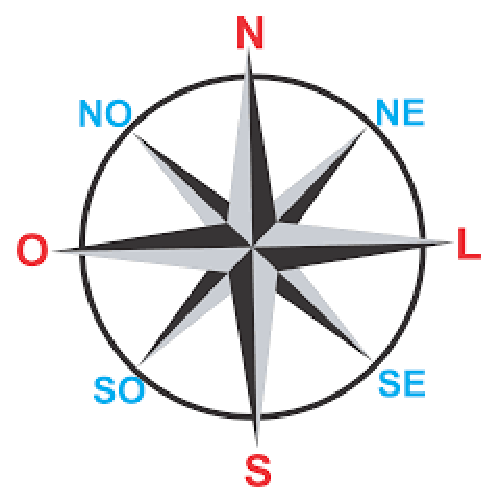
\includegraphics[width = 4.5 cm]{rosadosventos}
  \caption{Sinaliza\c{c}\~ao dos sentido cardeias da Rosa-dos-Ventos. Fonte~\cite{rosadosventos}.}
  \label{fig:rosadosventos}
\end{figure}

Considerando um subconjunto $S$ de imagem, dois~\textit{pixels} pertencentes a $S$ s\~ao conectados, considerando um dos crit\'erios de adjac\^encia, caso exista um caminho entre eles que tamb\'em perten\c{c}a a $S$. Para qualquer~\textit{pixel} $p$ em $S$, o conjunto de~\textit{pixels} que proporciona a uni\~ao a $q$ \'e denominado de~\textit{conjunto conectado}. Caso $q$ seja adjacente a $p$, este \'e chamado de~\textit{componente conectado}.

Uma regi\~ao $R$ \'e definida como um conjunto conectado e o contorno $C$ de $R$ \'e definido como sendo os~\textit{pixels} que possuem vizinhos que tanto pertencem $R$ como n\~ao pertencente.


\subsection{M\'edia Aritm\'etica e Desvio Padr\~ao}
Uma das formas de mensurar o comportamento de fen\^omenos ao longo do tempo - considerando o tempo como a generaliza\c{c}\~ao para a vari\'avel independente do fen\^omeno e n\~ao apenas como o tempo decorrido em, por exemplo, segundos - \'e atrav\'es da~\textit{m\'edia aritm\'etica} ($M_e(X)$). Como foi definido anteriormente, uma imagem \'e uma fun\c{c}\~ao discreta e para tal \'e poss\'ivel definidir a m\'edia aritm\'etica como sendo o somat\'orio das intensidades dos~\textit{pixels} dividido pela quantidade de~\textit{pixels} somados, tendo a express\~ao geral:
$$M_e(X) = {{x_1 + x_2 + ... + x_n} \over {n}}  = {{{1} \over {n}} \sum\limits_{i = 1}^{n}x_i},$$
onde $x_1$,$x_2$, ..., $x_n$ s\~ao as intensidades observadas nos~\textit{pixels} de estudo.

Al\'em da $M_e(X)$, a estat\'istica fornece v\'arias ferramentas para a representa\c{c}\~ao da variabilidade de um conjunto de dados, uma vez que grupos distintos podem apresentar a mesma m\'edia; neste projeto ser\'a utilizada a ferramenta denominada~\textit{desvio padr\~ao} ($D_P(X)$), tendo a express\~ao geral:
$$D_P(X) = \sqrt{{{1} \over {n}} \sum\limits_{i = 1}^{n}(x_i - M_e(X))^2}$$

\subsection{Espa\c{c}o de Cores}
As imagens coloridas s\~ao constru\'idas atrav\'es de espa\c{c}os de cores, por exemplo o~\textit{RGB} (\textit{Red, Green e Blu} ou, em portugu\^es, Vermelho, Verde e Azul). Os monitores de computadores e~\textit{smartphones}, al\'em dos televisores, s\~ao constituidos por v\'arios~\textit{pixels}, como demostrado na Figura~\ref{fig:monitorpixel}, sendo que cada~\textit{pixel} \'e constituido por $3$~\textit{LEDs}, basicamente, para cada cor do~\textit{RGB}.

Considerando que cada~\textit{pixel} em cada plano de um espa\c{c}o de cores \'e descrito por $1$~\textit{byte} ou $8$~\textit{bits}; ao implementar este conhecimento no espa\c{c}o de cores~\textit{RGB} \'e poss\'ivel ter $256^3$ cores diferentes. Mesmo tendo esta grande gama de cores \'e sabido que o olho humano \'e mais sens\'ivel \`a lumin\^ancia (brilho) do que \`a cor; considerando que o RGB, em que a lumin\^ancia est\'a espalhada pelas componentes, n\~ao \'e adaptado para se aproximar da sensibilidade humanda \'e preciso utilizar outro espa\c{c}o de cores que fa\c{c}a tal adapta\c{c}\~ao.

Como op\~ao tem o espa\c{c}o de cores~\textit{YCbCr} que possui as componentes: lumin\^ancia (Y) e as cromin\^ancias (Cb e Cr), onde a lumin\c{C}\^ancia \'e mais significativa do que as cromin\^ancias.

\'E importante ressaltar que, devido \`a constitui\c{c}\~ao dos monitores, e similares, \'e necess\'ario que haja formas de convers\~ao entre os espa\c{c}os de cores, independente de qual seja o escolhido, para o padr\~ao~\textit{RGB}; \'e poss\'ivel tal convers\~ao entre o~\textit{RGB} e o~\textit{YCbCr}.

\begin{figure}[]
  \centering
  
\includegraphics[width = 4.5 cm]{monitorpixel}
  \caption{Aproxima\c{c}\~ao num monitor, sendo poss\'ivel perceber os~\textit{pixels} e os~\textit{LED} do espa\c{c}o de cor~\textit{RGB}. Fonte~\cite{monitor}.}
  \label{fig:monitorpixel}
\end{figure}

\subsection{F-Measure ($F_1$)}
Em an\'alise estat\'istica de classifica\c{c}\~ao bin\'aria, o $F_1$ \'e a medida de acur\'acia de testes, precis\~ao; considera tanto os verdadeiros positivos ($P_V$) como os falsos ($P_N$), possuindo como resultado um valor entre $0$ e $1$ respeitando a rela\c{c}\~ao: (pior) $0 \leq resultado \geq 1$ (melhor), pela express\~ao geral:
$$F_1 = \left[{{2P_V} \over {2P_V + P_N}}\right]$$



\section{Metodologia}
Com as defini\c{c}\~oes feitas \'e poss\'ivel prosseguir para o desenvolvimento do projeto. Para tanto foram utilizados alguns recursos disponibilizados pela~\textbf{\textit{OpenCV}}~\cite{opencv}~(\textit{Open Source Computer Vision Library} ou, em portugu\^es, Biblioteca de Vis\~ao Computacional em C\'odigo Aberto). O projeto foi dividido em etapas:

\subsection{Constru\c{c}\~ao da Paleta de Cores}
Para que haja a caracteriza\c{c}\~ao de cor de pele \'e importante tem uma base de compara\c{c}\~ao; como o banco de dados \'e compartilhado por toda a turma, foi definido que as $20$ imagens fossem destinadas para a constru\c{c}\~ao da paleta, seguindo o crit\'erio que deva conter $10$ fotos de cada classe, sendo, ainda, estas subdivididads em $5$ de cada g\^enero, e que estas fotos sejam as mesmas para toda turma, diferenciando, somente, quanto aos peda\c{c}os de pele a serem recortados, o resultado \'e demonstrado na Figura~\ref{fig:paleta}.

\begin{figure}[!t]
  \centering
  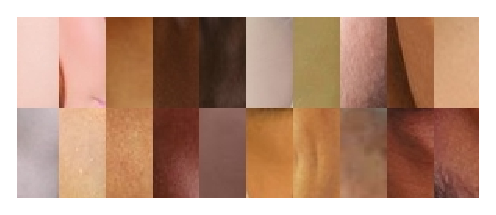
\includegraphics[width = 4.5 cm]{Paleta}
  \caption{Paleta desenvolvida com recortes de pele de imagens, base para a compara\c{c}\~ao.}
  \label{fig:paleta}
\end{figure}

Procurou-se construir uma paleta que continha transi\c{c}\~ao entre os tons de pele, dentro de cada imagem, pois dessa forma a gama de tons caracter\'isticos como tons de pele seria um grupo com menos restri\c{c}\~oes que as j\'a impostas.

A partir da paleta de cores foram definidos as m\'edias aritm\'eticas e os desvios padr\~oes para o espa\c{c}o de cores~\textit{YCbCr}, sendo este os valores de refer\^encia para as futuras compara\c{c}\~oes.

\subsection{Binariza\c{c}\~ao das imagens}
Com a constru\c{c}\~ao da paleta de cores, o passo seguinte \'e a binariza\c{c}\~ao das imagens.

Para tal tarefa foi realizada a convers\~ao de espa\c{c}os de cores, do~\textit{RGB} para o~\textit{YCbCr}, pois uma pele n\~ao deixa de ser uma pele com a varia\c{c}\~ao de luminosidade. Ap\'os isso, os~\textit{pixels} de cada plano de cromin\^ancia foram comparados com os valores determinados pela paleta de cores; caso estive no intervalo m\'edia $\pm$ desvio padr\~ao, ent\~ao era marcado como $1$ (branco) ou $0$ (preto), caso contr\'ario. Dessa forma, a imagem \'e binarizada com rela\c{c}\~ao a cor de pele.

Os planos de cromin\^ancia do~\textit{YCbCr} podem sofrer opera\c{c}\~oes de redimensionamento sem altera\c{c}\~ao ao olho nu, por isso as imagens foram redimensionadas para $400 \times 400$, para agilizar o processamento do banco de dados.

\subsection{Detec\c{c}\~ao das Regi\~oes}
O algoritmo adotado para a deterc\c{c}\~ao das regi\~oes considera a conectividade entre os~\textit{pixels}, uma vez que para tal tarefa seguiu-se os passos:

\begin{enumerate}
 \item Encontre um~\textit{pixel} branco, marque-o como visitado e armazene-o como sendo o piv\^o de uma regi\~ao;
 \item Busque na vizinhan\c{c}a de 8 se h\'a outros~\textit{pixels} brancos;
    \begin{enumerate}
     \item Caso encontre, marque-o como visitado e armazene-o na regi\~ao do seu~\textit{pixel} piv\^o correspondente;
	\begin{enumerate}
	 \item Repita a partir do passo $2)$.
	\end{enumerate}
     \item Repita enquanto houver~\textit{pixel} a ser visitado ou n\~ao houver mais~\textit{pixels} conectados a esta regi\~ao;
    \end{enumerate}
 \item Repita enquanto houver imagem a ser navegada.
\end{enumerate}

Esta maneira de procurar as regi\~oes deriva das~\textit{buscas em largura e profundidade} em~\textit{grafos}, visto que busca de maneira recursiva os~\textit{pixels} conectados \`a regi\~ao a partir de um dado~\textit{pixel} piv\^o.

\subsection{Classifica\c{c}\~ao das imagens}
Al\'em das imagens a serem classificadas houve imagens de treinamento, com caracter\'isticas semelhantes \`as imagens a serem classificadas - tamb\'em compartilhadas com a turma. Isto foi feito para que se tenha um crit\'erio quanto a discrimina\c{c}\~ao entre as classes.

Para as imagens de treinamento foram feitos os mesmos procedimento que seriam feitos com as imagens a serem classificadas; a diferen\c{c}a est\'a no fato de que foi calculado a m\'edia da \'area dita como pele para ambas as classes, dessa forma foi calculada a m\'edia das m\'edias para a determina\c{c}\~ao da m\'edia limiar para a distin\c{c}\~ao entre as classes.

\subsection{C\'alculo da F-Measure}
Com a constru\c{c}\~ao da m\'edia limiar entre as classes, foi poss\'ivel realizar a distin\c{c}\~ao entre as classes para as imagens lidas, ao passo que s\~ao contados os verdadeiros positivos.

\section{Resultados}
Houve imagens classificadas corretamente entre as classes, considerados como os verdadeiros positivos, como demonstrado na Figura~\ref{fig:vddpos}, tendo como origem a Figura~\ref{fig:vddposf}; ao passo que, tamb\'em, houve erros quanto a classifica\c{c}\~ao entre as classes, considerados como os falsos positivos, como demonstrado na Figura~\ref{fig:fkpos}, tendo como origem a Figura~\ref{fig:fkposf}, oriundo da falha de binariza\c{c}\~ao, comentada a seguir. Apesar disso, o algoritmo possui um~\textit{F-Measure} de $0.745645$.

Houve problemas em algumas imagens quanto a binariza\c{c}\~ao, como demonstrados nas Figuras~\ref{fig:fk}, tendo como origem a Figura~\ref{fig:fkf}, pois, visualmente, \'e de conhecimento geral que se tratava de uma representa\c{c}\~ao de uma pessoa na imagem, mas quanto aos valores dos~\textit{pixels}, a maioria foge da m\'edia estabelecida pela paleta; houve o acr\'escimo aos valores das m\'edias e dos desvios padr\~oes, a fim de minimizar este erro de reconhecimento de tom de pele.

Um aspecto positivo para o algoritmo desenvolvido \'e a rapidez que processa as imagens, visto que foram lidas pouco mais de $200$ imagens em menos de $15$ segundos de processamento.

\begin{figure}[!t]
  \centering
  
\includegraphics[width = 4.5 cm]{vddpos}
  \caption{Imagen classificada como verdadeiro positivo.}
  \label{fig:vddpos}
\end{figure}

\begin{figure}[!t]
  \centering
  \includegraphics[width = 4.5 cm]{vddposf}
  \caption{Original da Figura~\ref{fig:vddpos}.}
  \label{fig:vddposf}
\end{figure}

\begin{figure}[!t]
  \centering
  
\includegraphics[width = 4.5 cm]{fkpos}
  \caption{Imagen classificada como falso positivo.}
  \label{fig:fkpos}
\end{figure}

\begin{figure}[!t]
  \centering
  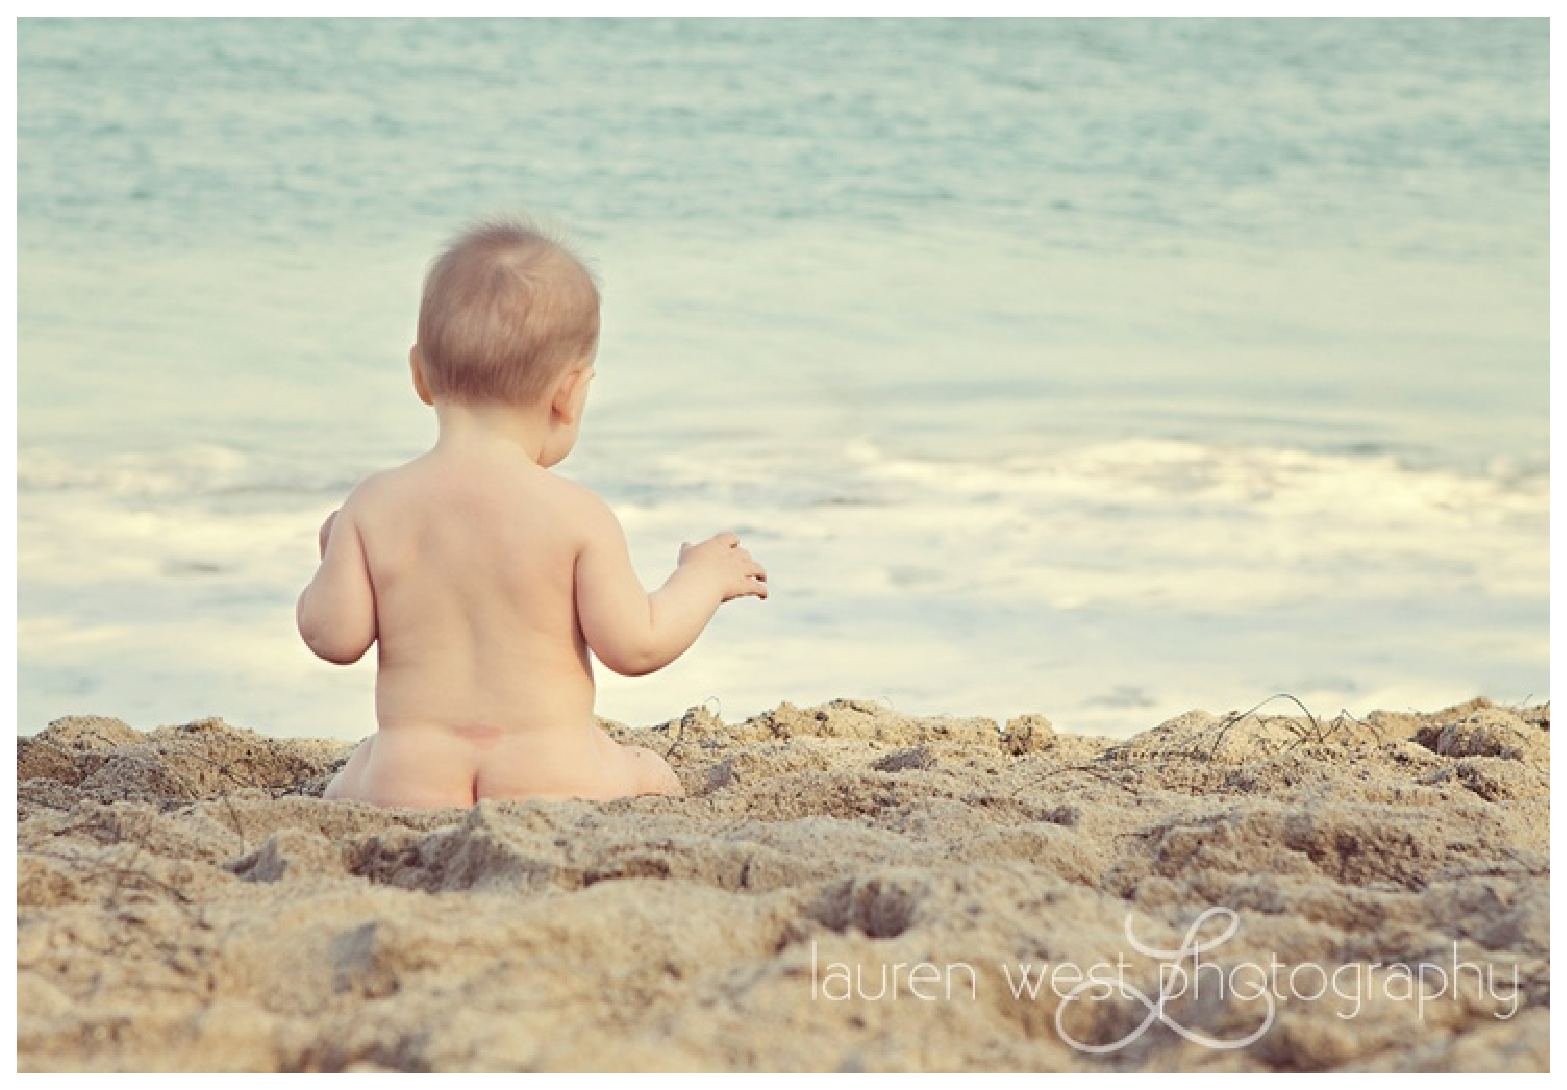
\includegraphics[width = 4.5 cm]{fkposf}
  \caption{Original da Figura~\ref{fig:fkpos}.}
  \label{fig:fkposf}
\end{figure}

\begin{figure}[!t]
  \centering
  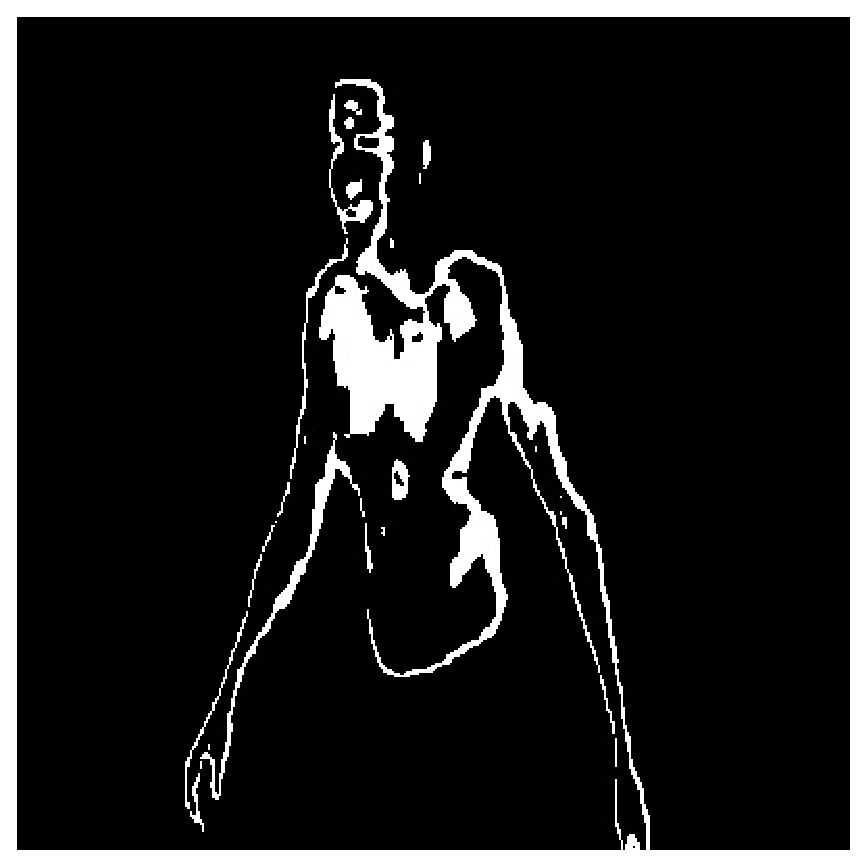
\includegraphics[width = 4.5 cm]{fk}
  \caption{Problema na binariza\c{c}\~ao.}
  \label{fig:fk}
\end{figure}

\begin{figure}[!t]
  \centering
  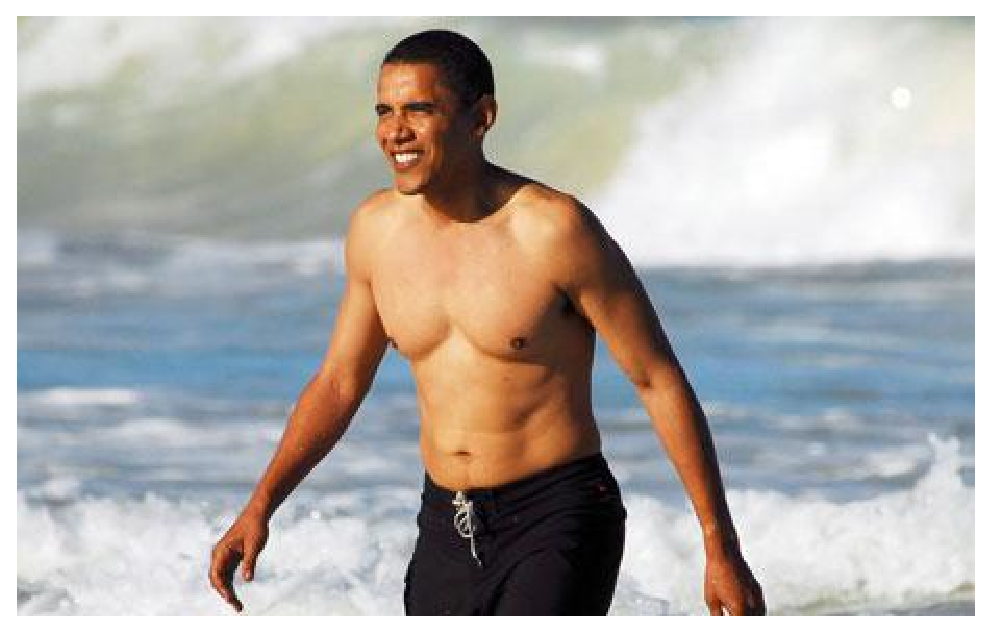
\includegraphics[width = 4.5 cm]{fkf}
  \caption{Original da Figura~\ref{fig:fk}.}
  \label{fig:fkf}
\end{figure}

\section{Conclus\~ao}
Este trabalho proporcionou uma maior fixa\c{c}\~ao do conte\'udo ministrado em sala de aula, uma vez que foi necess\'ario o desenvolvimento de todo o algoritmo.

Al\'em disso, com o valor de $0.745645$ para o~\textit{F-Measure}, conclui-se que o projeto mesmo com limiti\c{c}\~oes quanto \`a correta classifica\c{c}\~ao das imagens, decorrente de falhas na binariza\c{c}\~ao das imagens, possui espa\c{c}o para que seja melhorado em atividades futuras.





% trigger a \newpage just before the given reference
% number - used to balance the columns on the last page
% adjust value as needed - may need to be readjusted if
% the document is modified later
%\IEEEtriggeratref{8}
% The "triggered" command can be changed if desired:
%\IEEEtriggercmd{\enlargethispage{-5in}}

% references section

% can use a bibliography generated by BibTeX as a .bbl file
% BibTeX documentation can be easily obtained at:
% http://www.ctan.org/tex-archive/biblio/bibtex/contrib/doc/
% The IEEEtran BibTeX style support page is at:
% http://www.michaelshell.org/tex/ieeetran/bibtex/
%\bibliographystyle{IEEEtran}
% argument is your BibTeX string definitions and bibliography database(s)
%\bibliography{IEEEabrv,../bib/paper}
%
% <OR> manually copy in the resultant .bbl file
% set second argument of \begin to the number of references
% (used to reserve space for the reference number labels box)
\begin{thebibliography}{1}

\bibitem{IEEEhowto:kopka}
H.~Kopka and P.~W. Daly, \emph{A Guide to \LaTeX}, 3rd~ed.\hskip 1em plus
  0.5em minus 0.4em\relax Harlow, England: Addison-Wesley, 1999.
\bibitem{Gonzalez}
Gonzalez, Rafael C. e Woods, Richard E.,\emph{Digital Image Processing}, 3$^o$ ed,
Pearson Ed. - ISBN: 9780131687288. 

\bibitem{Gonzalez}
Bussab, Wilton de Oliveira; Morettin, Pedro Alberto, \emph{Estat\'itica B\'asica}, 8$^o$ ed,
Editora Saraiva - ISBN: 9788502207998

\bibitem{opencv}
Documentation, OpenCV. \emph{Welcome to opencv documentation}. Dispon\'ivel em: $http://docs.opencv.org/index.html$, acessado em 2015.

\bibitem{monitor}
One Climbs.\emph{Three: The Exploration of Archetypal Symbols Series}. Dispon\'ivel em:
$http://oneclimbs.com/2011/03/14/three-the-exploration-of-archetypal-symbols-series/$, acessado em 2015.

\bibitem{rosadosventos}
Tr\'iade da Aprova\c{c}\~ao.\emph{N\'iveis de Conhecimento: Por onde come\c{c}ar e at\'e onde voc\^e deve estudar cada assunto?}. Dispon\'ivel em:
$http://triadedaaprovacao.com/niveis-de-conhecimento-por-onde-comecar-e-ate-onde-voce-deve-estudar-cada-assunto/$, acessado em 2015;


\end{thebibliography}




% that's all folks
\end{document}